\documentclass[12pt]{article}
\usepackage{lineno}
\usepackage[spanish]{babel}
\usepackage{amsmath}
\usepackage{graphicx}
\usepackage[utf8]{inputenc}
\usepackage{pslatex}
\usepackage{theorem}
\newtheorem{teorema}{Teorema}
\newtheorem{proposicion}{Proposición}
\newtheorem{nota}{Nota}
\DeclareGraphicsExtensions{.pdf,.png,.jpg}

\author{Exequiel Aguirre}
\title{Estrategias de determinante cero de W.H. Press y F.J. Dyson}
\date{}
% document start
\begin{document}
%\linenumbers
\maketitle

\begin{abstract}
El juego del dilema del prisionero, en su versión de dos jugadores, puede ser usado como modelo para 
muchas situaciones del mundo real que involucran cooperativismo. Se asume en general, que no hay una estrategia
donde, unilateralmente, se pueda forzar a recibir una recompensa injusta.
En el artículo publicado por W.H. Press y F.J. Dyson, se muestra que existen estrategias con esa característica.
Con dichas estrategias, un jugador puede forzar el puntaje del oponente o establecer una relacion lineal entre
el puntaje propio y el del oponente.
\end{abstract}




\section{Introducción}
El dilema del prisionero provee de  marco para entender como dar con un balance entre cooperación y competencia, y es
a su vez una herramienta muy útil para tomar deciciones estratégicas.
Es por esto que tiene aplicaciones en diversas areas, como por ejemplo:Economía,política,biología,psicología y sociología.
El juego consiste en lo siguiente:
Si X e Y cooperan, ambos ganan una recompensa R.Si uno de ellos no coopera,recibe un pago mayor T, mientras que el
jugador que coopera recibe una recompensa menor, S, usualmente cero. Si ambos no cooperan, entonces reciben una recompensa P.
Para que el juego sea de interes, se debe satisfacer que $T >  R > P > S$ y $R > T+S$.
Los valores convencionales son (T,R,P,S)=(5,3,1,0)
\begin{center}
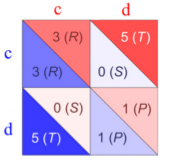
\includegraphics[height=3cm]{./pd.png}
\end{center}


El dilema del prisionero iterado, consiste en sucesivas partidas jugadas por, digamos X e Y.
Aquí los jugadores podrían basar sus jugadas en las jugadas anteriores.Sería natural pensar que el jugador que es
capaz de recordar más jugadas, podría confeccionar una estrategias más eficiente y así llevar ventaja.
Se va a probar luego, que esto no es así, y que solo importa la última jugada. Es por eso que las estrategias seran elaboradas
a partir de el último resultado, sin pérdida de generalidad.
Es decir, cada jugador va a basar su estrategia en el resultado xy $\in$ (cc,cd,dc,dd) donde c significa cooperar y d, no cooperar 
(defect en inglés). La estrategia de X, p=($p_1,p_2,p_3,p_4$) son las probabilidades de cooperar en cada una de las situaciones 
anteriores. En forma análoga, la estrategia de Y es q=($q_1,q_2,q_3,q_4$) visto desde su perspectiva yx $\in$ (cc,cd,dc,dd).

\section{Resultados}
\subsection{Estrategias de determinante cero}
Si bien es posible realizar una simulación del juego, movimiento por movimiento,uno podría evitar esto, con una matriz de
de transición de Markov.Esta matriz es generada a partir de las estrategias p y q.
$$M=
\begin{bmatrix}
 p_1 q_1 &p_1(1-q_1) &(1-p_1)q_1 &(1-p_1)(1-q_1)\\
 p_2 q_3 &p_2(1-q_3) &(1-p_2)q_3 &(1-p_2)(1-q_3)\\
 p_3 q_2 &p_3(1-q_2) &(1-p_3)q_2 &(1-p_3)(1-q_2)\\
 p_4 q_4 &p_4(1-q_4) &(1-p_4)q_4 &(1-p_4)(1-q_4)\\
\end{bmatrix}
$$
El valor $M_{ij}$ representa la probabilidad de pasar de un estado i a un estado j donde, i,j estan asociados a una 
estrategia en (cc,cd,dc,dd), según la perspectiva de cada jugador.
Por ejemplo, $M_{32}$ representa la probabilidad de pasar de un estado dc a cd.
Un vector estacionario v es aquel tal que:
\begin{center}
$v^T M = v^T$
\end{center}
Es decir, un autovector (a izquierda) asociado al autovalor 1.
Con v y el vector de pagos asociado a cada jugador, uno puede calcular el resultado del juego.

Dado que M tiene un autovector asociado al autovalor 1, la matriz M':=M-I es singular y por ende, de 
determinante cero.
Si se aplica la regla de Cramer a la matriz M', se obtiene
\begin{center}
$Adj(M')M' = det(M')I=0$
\end{center}
Sea A:=Adj(M'), entonces por la igualdad anterior, tenemos que:
\begin{center}
$AM'=A(M-I)=0 => AM=A$
\end{center}
Es decir, que el elemento 
\begin{center}
$(AM)_{ij}=\sum_{k=1}^4 A_{ik} M_{kj} = A_{ij}$
\end{center}
Ahora, sea w la n-esima fila de A.
\begin{center}
$w:=(w_1,w_2,w_3,w_4)=(A_{n1},A_{n2},A_{n3},A_{n4})$
\end{center}
Entonces, el j-esimo elemento del vector (w M) es,
\begin{center}
$(w M)_j=\sum_{k=1}^4 w_k M_{kj} =\sum_{k=1}^4 A_{nk} M_{kj} = A_{nj}=w_j$
\end{center}
Es decir que w M= w, por ende, w es proporcional a v.
Dado que n es arbitrario, se puede concluir que cada fila de Adj(M') es proporcional a v

Sea w, la cuarta fila de la matriz A, 
\begin{center}
$w:=(w_1,w_2,w_3,w_4)=(A_{41},A_{42},A_{43},A_{44})$.
\end{center}
Nos enfocaremos en la primera componente de w, por un momento.
\begin{center}
 $$
 w_1=A_{41}=Adj(M')_{41}=(-1)^{4+1} C_{14}=- det
 \begin{bmatrix}
 p_2 q_3 & p_2(1-q_3)-1 &(1-p_2)q_3 \\
 p_3 q_2 & p_3(1-q_2) &(1-p_3)q_2 -1 \\ 
 p_4 q_4 & p_4(1-q_4) &(1-p_4)q_4 \\ 
 \end{bmatrix}
 $$
 \end{center}
 Donde $(-1)^{4+1} C_{14}$ es el cofactor de $M'_{41}$. Este determinante no se modifica si sumamos la 
 primera columna de M' a la segunda y tercera, obteniendo
 \begin{center}
 $$w_1=- det
 \begin{bmatrix}
 p_2q_3 & p_2(1-q_3)-1+p_2q_3 &(1-p_2)q_3+p_2q_3 \\
 p_3q_2 & p_3(1-q_2)+p_3q_2 &(1-p_3)q_2 -1+p_3q_2 \\ 
 p_4q_4 & p_4(1-q_4)+p_4q_4 &(1-p_4)q_4+p_4q_4 \\ 
 \end{bmatrix}
 =- det
 \begin{bmatrix}
 p_2q_3 & p_2-1 & q_3 \\
 p_3q_2 & p_3 & q_2-1 \\ 
 p_4q_4 & p_4 & q_4 \\ 
 \end{bmatrix} 
 $$
\end{center} 
Llamemos $W_1$ a esta última matriz.Un cálculo similar se puede realizar y obtener matrices $W_2,W_3,W_4$ 
correspondientes a $w_2,w_3,w_4$ respectivamente. Es decir que las componentes de v, son salvo un signo, 
determinantes de una matriz de este tipo.
Ahora sea, $f=(f_1,f_2,f_3,f_4)$,entonces,
\begin{center}
$$
D(p,q,f):=det
\begin{bmatrix}
 p_1q_1-1 & p_1-1 & q_1-1 & f_1 \\
 p_2q_3 & p_2-1 & q_3 & f_2\\
 p_3q_2 & p_3 & q_2-1  & f_3\\ 
 p_4q_4 & p_4 & q_4 & f_4\\ 
 \end{bmatrix} 
 $$
 $$
 =-det(W_1)f_1 +det(W_2)f_2 -det(W_3)f_3 +det(W_4)f_4 
 = v \cdot f
 $$
\end{center}
Notar que la segunda columna $\tilde{p}= (p_1-1,p_2-1,p_3,p_4)$ está solo bajo el control de X.
Analogamente la tercera columna $\tilde{q}=(q_1-1,q_3,q_2-1,q_4)$ esta bajo el control de Y.
Sean $S_X:=(R,S,T,P)$ , $S_Y:=(R,T,S,P)$ los vectores de pago de X e Y respectivamente.
En su estado estacionario, podemos escribir los respectivos puntajes finales, como:
\begin{center}
$s_X=\frac{v \cdot S_X}{v \cdot \overline1} = \frac{D(p,q,S_X)}{D(p,q,\overline1)}$ , 
$s_Y=\frac{v \cdot S_Y}{v \cdot \overline1} = \frac{D(p,q,S_Y)}{D(p,q,\overline1)}$
\end{center}
Donde el vector $\overline1:=(1,1,1,1)$.Estos denominadores son necesarios para que sus
componentes sumen 1, (requerido en un para un vector de probabilidad estacionario)
Dado que los puntajes s, dependen linealmente de los vectores de pago S, lo mismo
sucede para una combinación lineal de los mismos.
\begin{center}
 $\alpha s_X + \beta s_Y + \gamma=\frac{D(p,q,\alpha S_X + \beta S_Y + \gamma\cdot \overline1)}{D(p,q,\overline1)}$
\end{center}
Esta es de alguna manera la ecuación más importante, pues tanto X como Y pueden elegir una
estrategia que anule el numerador. Es decir, si X elije una estrategia 
$\tilde{p}= \alpha S_X + \beta S_Y + \gamma\cdot \overline1$, o si Y elije una estrategia
$\tilde{q}= \alpha S_X + \beta S_Y + \gamma\cdot \overline1$ entonces 

\begin{center}
$\alpha s_X + \beta s_Y + \gamma$=0
\end{center}
Estas son las llamadas, estrategias de determinante cero.

\subsection{X define unilateralmente el puntaje de Y}
Un caso particular de una estrategia de determinante cero, es donde X define el puntaje de Y.
Eligiendo $\alpha=0$ en la ecuación anterior, obtenemos: $\tilde{p}=\beta S_Y + \gamma \overline1$
Esto nos define cuatro ecuaciones:
$$p_1-1=\beta R + \gamma$$
$$p_2-1=\beta T + \gamma$$
$$p_3=\beta S + \gamma$$
$$p_4=\beta P + \gamma$$
Eliminando $\beta$ y $\gamma$, obtenemos,
$$p_2=\frac{p_1(T-P)-(1-p_4)(T-R)}{R-P}$$
$$p_3=\frac{(1-p_1)(P-S)+p_4(R-S)}{R-P}$$
$$s_Y=\frac{-\gamma}{\beta}=\frac{\beta R+ 1-p_1}{\beta}=\frac{(1-p_1)P+p_4 R}{p_4-p_1+1}$$
De esta última ecuación, se desprende que X puede forzar el puntaje de Y,
$$P\leq s_Y\leq R $$

\subsection{X intenta definir su propio puntaje}
Analogamente al caso anterior,con $\tilde{p}=\alpha S_X + \gamma\overline1$  obtenemos,
$$p_2=\frac{(1+p_4)(R-S)-p_1(P-S)}{R-P}\geq 1$$
$$p_3=\frac{-(1-p_1)(T-P)-p_4(T-R)}{R-P}\leq 0$$
Estas ecuaciones nos indican que la única estrategia posible es p=(1,1,0,0), es decir
X no puede decidir su puntaje unilateralmente.


\subsection{X demanda y obtiene una porción del puntaje de Y}
El jugador X, ahora pretende establecer una relación lineal entre su puntaje y el de Y,
$$(s_X -P)=\chi (s_y-P)$$
con $\chi \geq 1$ (para así beneficiarse). Equivalentemente,
$$(s_X -P)-\chi (s_y-P)=0 <=>\phi[(s_X -P)-\chi (s_y-P)]=0 <=>\frac{\phi}{P-S}[(s_X -P)-\chi (s_y-P)]=0$$
Con $\phi>0$. X puede forzar esta relación eligiendo la estrategia
$$\tilde{p}=\frac{\phi}{P-S}[(S_X-P\cdot\overline1)\ - \chi (S_Y-P\cdot\overline1)]$$
Así obtenemos,
$$p_1=1-\frac{\phi}{P-S}(R-P)(\chi-1)$$
$$p_2=1-\phi(1+\chi \frac{T-P}{P-S})$$
$$p_3=\phi(\frac{T-P}{P-S}+\chi )$$
$$p_4=0$$
De la ecuación de $p_2$ se puede verificar que,
$$\phi(1+\chi\frac{T-P}{P-S})\leq 1 => \phi\leq(1+\chi \frac{T-P}{P-S})^{-1}=\frac{P-S}{(P-S) + \chi(T-P)}$$
Ahora el puntaje de X depende del puntaje de Y.Ambos son máximos cuando Y coopera plenamente, con
q=(1,1,1,1). En este caso, el puntaje de X es,
$$s_X= \frac{D(p,q,S_X)}{D(p,q,\overline1)}=\frac{(\chi R + (1-\chi)P)T-\chi RS+(\chi-1)PR}{T-\chi S+(\chi-1)R}=$$
$$\frac{P(T-R)+\chi[R(T-S)-P(T-R)]}{(T-R)+\chi(R-S)}$$
Esta situación se puede hacer más concreta, con los valores convencionales (T,R,P,S)=(5,3,1,0), entonces,
$$p=[1-2\phi(\chi-1),1-\phi(4 \chi+1),\phi(\chi+4),0]$$
Donde los mejores puntajes posibles para X e Y son,
$$s_X=\frac{2+13\chi}{2+3\chi}, s_Y=\frac{12+3\chi}{2+3\chi}$$
El parametro \chi es conocido como el factor de extorsión. En el caso particular donde, \chi=1 , y \phi =1/5
entonces la estrategia p=(1,0,1,0), la estrategia de tit-for-tat.



 \section{Bibliografía}
  \begin{thebibliography}{1}
  \end{thebibliography}


\end{document}



